%!TEX TS-program = pdflatex
% Booklet @ https://github.com/zfengg/Booklet
%
%	A simple TeX template to create booklets for conferences.
%
% Author: Zhou Feng @ 26/11/2023
% ---------------------------------------------------------------------------- %
%                                   preamble                                   %
% ---------------------------------------------------------------------------- %
\documentclass[openany,parskip=half,12pt,a4paper,table]{scrbook}
			  
% ------------------------------ input tex files ----------------------------- %
% !TEX root = ../booklet.tex
% ------------------------------- misc: prefix ------------------------------- %
\usepackage{scrhack} % fixes compatibilities
\usepackage{lastpage} % count total num of pages

% ----------------------------------- math ----------------------------------- %
\usepackage{amsmath,amsfonts,amssymb}
\usepackage{mathrsfs}
\usepackage{mathtools}
\allowdisplaybreaks

% ---------------------------------- layout ---------------------------------- %
\usepackage[top=2.5cm,bottom=2.5cm,inner=1.5cm,outer=3cm,
			footskip=1.4cm,headsep=0.8cm,headheight=0.5cm,
%			showframe, % for debugging
			]{geometry}
% \renewcommand{\baselinestretch}{1.5}
% equalize margins on odd and even pages
\setlength\oddsidemargin{\dimexpr(\paperwidth-\textwidth)/2 - 1in\relax}
\setlength\evensidemargin{\oddsidemargin}

% ------------------------------ header & footer ----------------------------- %
\pagestyle{plain}

% ----------------------------------- lists ---------------------------------- %
\usepackage{caption}
\usepackage[shortlabels,inline]{enumitem}
\setitemize{itemsep=0.6ex}

% ---------------------------------- tables ---------------------------------- %
\usepackage{multicol}
\usepackage{multirow}
\usepackage{longtable} % tables with multiple pages
\usepackage{array}
\renewcommand{\arraystretch}{1.5} % the spreadout of cells in tables

% column types
\newcolumntype{L}[1]{>{\raggedright\let\newline\\\arraybackslash\hspace{0pt}}m{#1}} % left-aligned
\newcolumntype{C}[1]{>{\centering\let\newline\\\arraybackslash\hspace{0pt}}m{#1}} % centred
\newcolumntype{R}[1]{>{\raggedleft\let\newline\\\arraybackslash\hspace{0pt}}m{#1}} % right-aligned

% ---------------------------------- figures --------------------------------- %
\usepackage{tikz}
\usepackage{tikz-cd}
\usepackage{float}
\usepackage{graphicx}
% cover page
\usepackage{eso-pic,contour}
\contourlength{.4pt}

% ------------------------------- fonts & input ------------------------------ %
\usepackage[utf8]{inputenc} 
\usepackage[T1]{fontenc}
\usepackage[sfdefault, lf]{carlito} % set font family
\usepackage{microtype} % improve typography

%% Chinese support by XeLaTeX
%\usepackage[scheme=plain]{ctex}
%%\usepackage{xeCJK} % Chinese via xelatex
%%\setCJKmainfont{SimSun}
%% \setCJKsansfont{SimSun}
%% \setCJKmonofont{SimSun}

% --------------------------------- numbering -------------------------------- %
\setcounter{secnumdepth}{-2} % rm section numbering

% ---------------------------------- colors ---------------------------------- %
\usepackage{xcolor}
% define
\definecolor{myorange}{RGB}{255, 117, 40}
\definecolor{mygray}{RGB}{164, 168, 172}
\definecolor{mywhite}{RGB}{235, 238, 231}
%\definecolor{myblue}{RGB}{52, 115, 116}
%\definecolor{myblue}{RGB}{0, 0, 128} % navy blue
\definecolor{myblue}{RGB}{0, 71, 171} % Cobalt Blue
% set main colors
\colorlet{colorMain}{myblue}
\newcommand{\colorMain}{myblue}
\newcommand{\colorBorderBar}{mywhite}
% colors in table
\newcommand{\tbg}{gray} % event background
\newcommand{\tfg}{white} % event foreground (text)
\newcommand{\tbc}{gray!20} % general background 

% ---------------------------- chapters & sections --------------------------- %
\RedeclareSectionCommand[afterskip=4em plus 1pt minus 1pt,beforeskip=-1pt,level=0,toclevel=0,]{chapter}
\RedeclareSectionCommand[afterskip=1pt,beforeskip=3pt,level=1,toclevel=1,]{section}

\newdimen\mybarpadding
\mybarpadding=1.5em\relax % padding between bar and chapter title
\renewcommand{\chapterlinesformat}[3]{%
	\ifthispageodd{% odd pages with bar on the left
		\hfill % Coloured bar fills available width
		\raisebox{-0.2em}{\makebox[0pt][r]{\textcolor{\colorMain}{\rule{\paperwidth}{1em}}}} % define the bar
		\hspace{\mybarpadding} % padding between bar and title
		\mbox{#3} % chapter title
	}{% even pages with bar on the right
		\mbox{#3} % chapter title
		\hspace{\mybarpadding} % padding between title and bar
		\raisebox{-0.2em}{\makebox[0pt][l]{\textcolor{\colorMain}{\rule{\paperwidth}{1em}}}} % color bar
	}%
}


% ----------------------- the vertical line in margins ----------------------- %
\usepackage{ifthen}
\usepackage[scale=1,angle=0,opacity=1]{background}
\backgroundsetup{contents={}}

\AddEverypageHook{%
	\ifthenelse{%
		\isodd{\thepage} \AND \thepage>1 \AND \NOT \thepage=\pageref{LastPage} % odd page but not the first or last
	}{%
		\backgroundsetup{
			color=\colorBorderBar, % set color
			position=current page.south east, % bar position on the page
			nodeanchor=south east, % anchor location inside the bar
			contents={\rule{10pt}{\paperheight}} % width and height of the bar
		}
	}{}
	%
	\ifthenelse{% 
		\NOT \isodd{\thepage} \AND \NOT \thepage=\pageref{LastPage} % If even page but not the last page
	}{%
		\backgroundsetup{
			color=\colorBorderBar, % set color
			position=current page.south west, % bar position on the page
			nodeanchor=south west, % anchor location inside the bar
			contents={\rule{10pt}{\paperheight}} % width and height of the bar
		}
	}{}
	%
%	\BgMaterial % output the above background setup
}

% -------------------------------- hyperlinks -------------------------------- %
\usepackage[pdfusetitle,
			bookmarks=true,
			pagebackref,
			hidelinks, % hide boxes surround links
			colorlinks=false,
			linkcolor=blue,
			citecolor=blue,
			urlcolor=blue]{hyperref}


% ---------------------------- categories of talks --------------------------- %
\newcommand{\circleGeneric}[2]{\tikz[baseline={([yshift=-.8ex]current bounding box.center)}]  \node[circle, inner sep=3pt, minimum size=0.5em, color=black, fill=#1]{\small \bfseries #2};} % tag icon
% invited speaker
\newcommand{\colorIS}{myblue!65}
\newcommand{\IS}[4]{#1 & \cellcolor{\colorIS}IS & {\bfseries#2}\newline #3 & & #4 \\ \hline}
\newcommand{\tagIS}{\circleGeneric{\colorIS}{IS}}
% contributed talk
\newcommand{\colorCT}{white}
\newcommand{\CT}[4]{#1 & \cellcolor{\colorCT} CT & {\bfseries#2}\newline #3 & & #4 \\ \hline}
\newcommand{\tagCT}{\circleGeneric{\colorCT}{CT}}
% keynote lecture
\newcommand{\colorKL}{myorange!45}
\newcommand{\KL}[4]{#1 & \cellcolor{\colorKL} KL & {\bfseries#2}\newline #3 & & #4 \\ \hline}
\newcommand{\tagKL}{\circleGeneric{\colorKL}{KL}}
% invited talk
\newcommand{\colorIT}{yellow!25}
\newcommand{\IT}[4]{#1 & \cellcolor{\colorIT} IT & {\bfseries#2} \newline #3 & & #4 \\ \hline}
\newcommand{\tagIT}{\circleGeneric{\colorIT}{IT}}

% rows in timetable
\newcommand{\rowBreak}[2]{ #1 & \cellcolor{\tbc} #2 \\ \hline}
\newcommand{\rowEvent}[2]{#1 & {\cellcolor{\tbg}\color{\tfg}\bfseries #2} \\ \hline}
\newcommand{\rowTalk}[4]{\multirow{2}{*}{#1} & #4 \\ & \textbf{#2}, \textit{#3} \\ \hline}
\newcommand{\rowThick}[2]{& \\ #1 & #2  \\ & \\ \hline}
\newcommand{\rowTHICK}[2]{\multirow{3}{*}{#1} & \\ & \\ & #2 \\ & \\ & \\ \hline}

% others
\newcommand{\tablebreak}[2]{\rowcolor{\tbc} #1 & \multicolumn{4}{c|}{\bfseries #2} \\ \hline }
\newcommand{\eventtype}[2]{#1 & \multicolumn{4}{c|}{\cellcolor{\tbg}\color{\tfg}\bfseries #2} \\ \hline }
\newcommand{\tutorial}[4]{#1 & & {\bfseries#2}\newline #3 & & #4 \\\hline}
\newcommand{\Talk}[4]{\multirow{2}{*}{#1}  & \multicolumn{4}{c|}{#4} \\ & \multicolumn{4}{c|}{\textbf{#2}, \textit{#1}} \\ \hline}
\newcommand{\TalkBreak}[4]{\pagebreak \hline \multirow{2}{*}{#1}  & \multicolumn{4}{c|}{#4} \\ & \multicolumn{4}{c|}{\textbf{#2}, \textit{#1}} \\ \hline}

% ---------------------------------- objects --------------------------------- %
% Abstract
\newcommand{\Abstract}[5][]{
	\filbreak % avoid pagebreaks
	
	{\large \bfseries #2}
	
%	\vskip -0.1em
	
	{\bfseries \itshape #3}, \textcolor{mygray}{#4} \hfill {#1}
	
%	\vskip -0.1em
	
	#5 % content
	\vskip 2em
} % end of Abstract

% Participant
\newcommand{\Participant}[2]{#1 & #2 \\} % name, affiliation

% Poster
\newcommand{\Poster}[3]{
	\filbreak % avoid page breaks
	{\large\bfseries #1}\\ % title
	\hspace*{0.75cm} #2, \textit{#3} % author, affiliation
}

% ------------------------------- misc: suffix ------------------------------- %
\usepackage[numbers,sort]{natbib} % sort citations
\usepackage{appendix}
\usepackage{pdfpages} % full-page image as cover

% !TEX root = ../booklet.tex

\usepackage{fix-cm}
\newcommand{\COVERPAGE}{%
	~\vskip 8em
	\sffamily
	{\fontsize{35}{50}\selectfont\selectfont\color{colorMain} International Conference on\\[5mm]
		Research Area \& Related Topics\\[15mm]
	}
		
	{\huge 11--15 December, 2023 \\[5mm]}
	
	{\huge Department, University \\[30mm]}

	\begin{center}
		\Huge\ttfamily Some Image
	\end{center}
	~\\[5mm]
} % end of COVERPAGE

% \makecover 
\newcommand{\makecover}{%
	\thispagestyle{empty}
	\AddToShipoutPictureFG*{%
		\begin{tikzpicture}[overlay]
			\node (A) at (current page.south west) {};
			\node (B) at ([xshift=20mm] current page.north west) {};
			\node (C) at ([xshift=20mm] current page.north west) {};
			\fill[colorMain] (A) rectangle (B);
			\node[anchor=north west,outer sep=5mm,inner sep=0pt] at (C) {\parbox{15cm}{\COVERPAGE}};
	\end{tikzpicture}}
	\hbox{}\newpage
} % end of \makecover % \makecover
% !TEX root = ../thesis.tex
% -------------------------------- fast-typing ------------------------------- %
% cali characters
\newcommand{\calF}{\mathcal{F}}
\newcommand{\calB}{\mathcal{B}}
\newcommand{\calP}{\mathcal{P}}
\newcommand{\calT}{\mathcal{T}}
\newcommand{\calD}{\mathcal{D}}
\newcommand{\calQ}{\mathcal{Q}}
\newcommand{\calR}{\mathcal{R}}
\newcommand{\calM}{\mathcal{M}}
\newcommand{\calL}{\mathcal{L}}
\newcommand{\calI}{\mathcal{I}}
\newcommand{\calG}{\mathcal{G}}
\newcommand{\calW}{\mathcal{W}}
% scurf characters
\newcommand{\scrB}{\mathscr{B}}
\newcommand{\scrD}{\mathscr{D}}
\newcommand{\scrP}{\mathscr{P}}
\newcommand{\scrA}{\mathscr{A}}
\newcommand{\scrE}{\mathscr{E}}
\newcommand{\scrC}{\mathscr{C}}
\newcommand{\scrT}{\mathscr{T}}
\newcommand{\scrQ}{\mathscr{Q}}
\newcommand{\scrF}{\mathscr{F}}
\newcommand{\scrG}{\mathscr{G}}
\newcommand{\scrW}{\mathscr{W}}
% blackboad characters
\newcommand{\bbQ}{\mathbb{Q}}
\newcommand{\bbR}{\mathbb{R}}
\newcommand{\bbC}{\mathbb{C}}
\newcommand{\bbZ}{\mathbb{Z}}
\newcommand{\bbN}{\mathbb{N}}
\newcommand{\bbP}{\mathbb{P}}
\newcommand{\bbT}{\mathbb{T}}
% frak characters
\newcommand{\frX}{\mathfrak{X}}
% rome characters
\newcommand{\rmN}{\mathrm{N}}
\newcommand{\rmR}{\mathrm{R}}
% math operators
\DeclareMathOperator*{\Lim}{Lim}
\DeclareMathOperator*{\llim}{\underline{lim}}
\DeclareMathOperator*{\ulim}{\overline{lim}}
\DeclareMathOperator*{\essinf}{ess\,inf}
\DeclareMathOperator*{\esssup}{ess\,sup}
\DeclareMathOperator*{\intersect}{\cap}
\DeclareMathOperator*{\Intersect}{\bigcap}
\DeclareMathOperator*{\union}{\cup}
\DeclareMathOperator*{\Union}{\bigcup}
\DeclareMathOperator{\ex}{ex}
\DeclareMathOperator{\co}{co}
\DeclareMathOperator{\diam}{diam}
\DeclareMathOperator{\supp}{supp}
\DeclareMathOperator{\Var}{Var}
\DeclareMathOperator{\Exp}{Exp}
\DeclareMathOperator{\Dim}{Dim}
\DeclareMathOperator{\ldim}{\underline{\dim}}
\DeclareMathOperator{\udim}{\overline{\dim}}
% commonly used
\newcommand{\Ndash}{\nobreakdash--}
\newcommand{\sigmaAlg}{$\sigma$\nobreakdash-algebra }
\providecommand{\abs}[1]{\lvert#1\rvert}
\providecommand{\Abs}[1]{\left\lvert#1\right\rvert}
\providecommand{\norm}[2][]{\lVert#2\rVert_{#1}}
\providecommand{\Norm}[2][]{\left\lVert#2\right\rVert_{#1}}
\newcommand{\ndiml}[1][n]{$#1$\nobreakdash-dim}
\newcommand{\padic}{$p$\nobreakdash-adic}
\newcommand{\kOrder}[1]{$#1$\nobreakdash-order}
\newcommand{\mDash}[2]{$#1$\nobreakdash-#2}
\newcommand{\euclid}[1][d]{\mathbb{R}^{#1}}
\newcommand{\innerprod}[2]{\langle #1, #2 \rangle}
\newcommand{\pairing}[2]{\left(#1, #2\right)}
\newcommand{\oneOver}[1]{\frac{1}{#1}}
\newcommand{\energy}[2][s]{I_{#1}(#2)}
\newcommand{\capacity}[2][s]{g_{#1}(#2)}
\newcommand{\wt}[1]{\widetilde{#1}}
\newcommand{\wh}[1]{\widehat{#1}}
\newcommand{\cl}[1]{\overline{#1}}
% dimensions
\newcommand{\dimH}{\dim_{\mathrm{H}}}
\newcommand{\dimP}{\dim_{\mathrm{P}}}
\newcommand{\dimB}{\dim_{\mathrm{B}}}
\newcommand{\dimC}{\dim_{\mathrm{C}}}
\newcommand{\dimF}{\dim_{\mathrm{F}}}
\newcommand{\dimE}{\dim_{\mathrm{e}}}
\newcommand{\dimsub}[1]{\dim_{\mathrm{#1}}}
\newcommand{\uDim}[1]{\overline{\dim}_{\mathrm{#1}}}
\newcommand{\lDim}[1]{\underline{\dim}_{\mathrm{#1}}}
\newcommand{\locDim}[2]{D(#1, #2)}
\newcommand{\ulocDim}[2]{\overline{D}(#1, #2)}
\newcommand{\llocDim}[2]{\underline{D}(#1, #2)}
\newcommand{\uTau}{\overline{\tau}}
\newcommand{\lTau}{\underline{\tau}}
% measures
\newcommand{\leb}[1]{\mathcal{L}(#1)}
\newcommand{\lebRes}[1]{\mathcal{L}\vert_{#1}}
\newcommand{\haus}[2]{\mathcal{H}^{#1}(#2)}
\newcommand{\hausC}[2]{\mathcal{H}^{#1}_{\infty}(#2)}
\newcommand{\hausO}[3]{\mathcal{H}^{#1}_{#2}({#3})}
\newcommand{\Haus}[1]{\mathcal{H}^{#1}}
\newcommand{\HausC}[1]{\mathcal{H}^{#1}_{\infty}}
\newcommand{\HausO}[2]{\mathcal{H}^{#1}_{#2}}
\newcommand{\pack}[2]{\mathcal{P}^{#1}(#2)}
\newcommand{\packP}[2]{\mathcal{P}^{#1}_{0}(#2)}
\newcommand{\packC}[3]{\mathcal{P}^{#1}_{#2}(#3)}
\newcommand{\Pack}[1]{\mathcal{P}^{#1}}
\newcommand{\PackP}[1]{\mathcal{P}^{#1}_{0}}
\newcommand{\PackC}[2]{\mathcal{P}^{#1}_{#2}}

% --------------------------------- meta info -------------------------------- %
\title{Title of Conference}
\author{First Last}

% ---------------------------------------------------------------------------- %
%                                   document                                   %
% ---------------------------------------------------------------------------- %
\begin{document}
	
% ----------------------------------- cover ---------------------------------- %
% 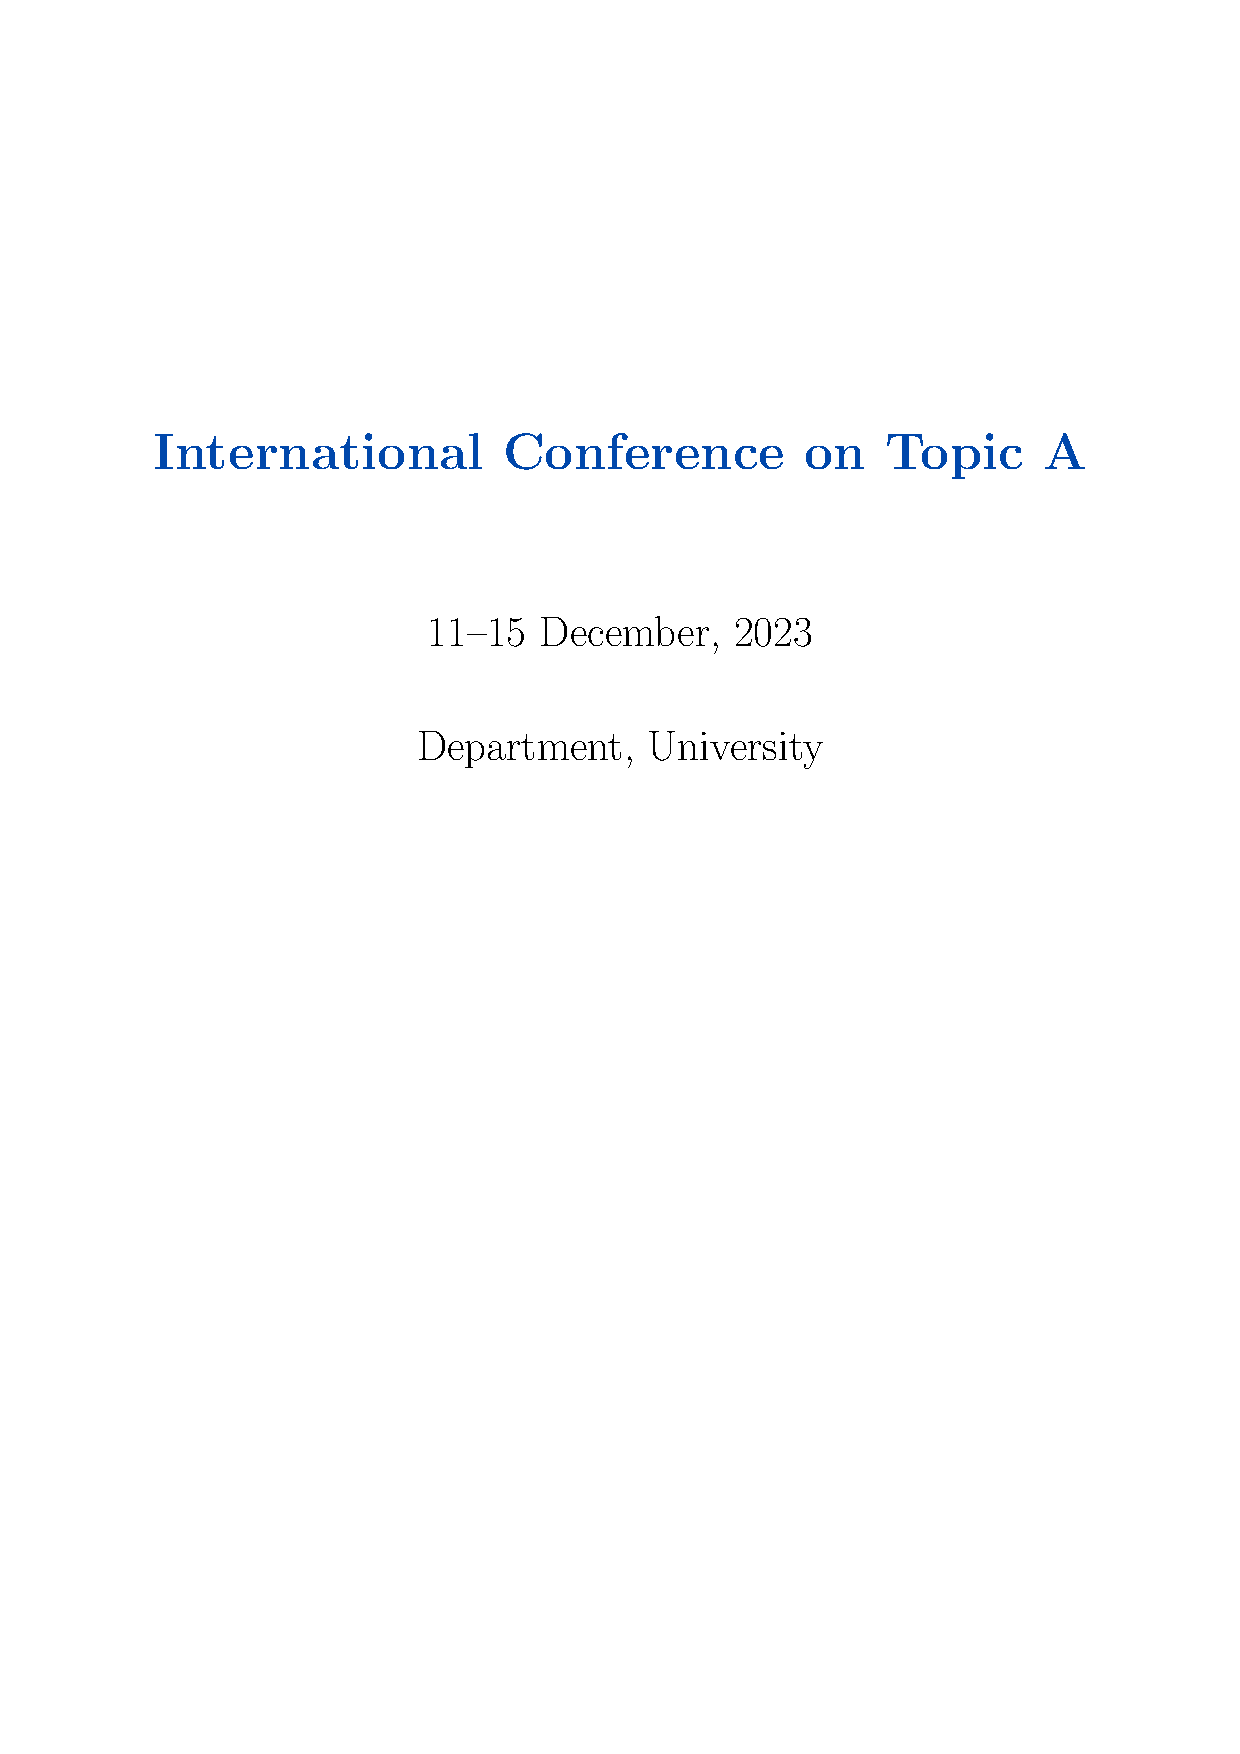
\includepdf{lib/cover.pdf}
\makecover

% ------------------------------- back of cover ------------------------------ %
\thispagestyle{empty}
~\vfill

\begin{center}
	This is a simple booklet generated using the template at:\\ \url{https://github.com/zfengg/Booklet}
\end{center}

\newpage

% ----------------------------- table of contents ---------------------------- %
\tableofcontents

% ----------------------------------- about ---------------------------------- %
\chapter{About}

{\small \textcolor{myblue}{This is a sample conference booklet for which this \LaTeX{} template was generated. Short documentations can be found at:\\ \url{https://github.com/zfengg/Booklet}}

\section{Title of the conference}

Some descriptions of the conference. The aim of this conference is to bring together scientists to discuss and exchange ideas on the cutting edge research on the area of ABC. The topics will include, for example, E on F, H, and I. It is in honor of Professor K.

\section{Scientific committee}
\begin{itemize}
	\item First Last (Affiliation)
	
	\item First Last (Affiliation)
	
	\item First Last (Affiliation)
\end{itemize}

\section{Organizing committee}
\begin{itemize}
	\item First Last (Affiliation)
	
	\item First Last (Affiliation)
	
	\item First Last (Affiliation)
\end{itemize}

\section{Enquiry}

\begin{description}
	\item[Email:] example@domain.com
	
	\item[Website:] \url{https://example.com}
	
	\item[Address:] Department, University, City, Country
\end{description}

\newpage

\section{Invited speakers}
\begin{itemize}
	\item First Last
	
	\item First Last
	
	\item First Last
\end{itemize}

% --------------------------------- timetable -------------------------------- %
\chapter{Timetable}

{\LARGE {\bfseries Venue:} Room 123 at Hall ABC.}

\section{11 December 2023, Monday}
\begin{longtable}{|C{0.15\textwidth}|C{0.7\textwidth}|}
	\hline
	\rowBreak{8:30--9:00}{Registration}
	\rowBreak{9:00--9:10}{Welcome remarks}
	\rowTalk{9:10--10:05}{Speaker}{Affiliation}{Title of the talk}
	\rowThick{}{Coffee Break/\textbf{Registration}}
	\rowTalk{14:00--14:30}{Speaker}{Affiliation}{Title of the talk}
	\rowTalk{14:30--15:05}{Speaker}{Affiliation}{Title of the talk}
	\rowBreak{15:05--15:30}{Coffee}
	\rowTalk{15:30-16:00}{Speaker}{Affiliation}{Title}
	\rowTalk{16:00-17:10}{Speaker}{Affiliation}{Title}
	\rowEvent{17:10--19:30}{Poster session with Wine \& Cheese}
\end{longtable}


\section{12 December 2023, Tuesday}
\begin{longtable}{|C{0.15\linewidth}| C{0.04\linewidth}|  C{0.3\linewidth} C{0.0\linewidth} C{0.4\linewidth}|}\hline
	\tablebreak{8:30--9:00}{Registration}
	\tablebreak{9:00--9:10}{Welcome remarks}
	\KL{9:10--10:05}{Speaker}{Affiliation}{Title}
	\IT{10:05--10:30}{Speaker}{Affiliation}{Title}
	\tablebreak{10:30--11:00}{Coffee}
	\IS{11:00--11:40}{Speaker}{Affiliation}{Title}
	\CT{11:40--12:45}{Speaker}{Affiliation}{Title}
	\tablebreak{12:45--14:00}{Lunch}
	\CT{14:00--14:30}{Speaker}{Affiliation}{Title}
	\IS{14:30--15:05}{Speaker}{Affiliation}{Title}
	\tablebreak{15:05--15:30}{Coffee}
	\CT{15:30-16:00}{Speaker}{Affiliation}{Title}
	\IS{16:00-17:10}{Speaker}{Affiliation}{Title}
	\eventtype{17:10--19:30}{Poster session with Wine \& Cheese}
\end{longtable}


\section{13 December 2023, Wednesday}
\begin{longtable}{|C{0.15\linewidth}| C{0.04\linewidth}|  C{0.3\linewidth} C{0.0\linewidth} C{0.4\linewidth}|}\hline
	\tablebreak{8:30--9:00}{Registration}
	\tablebreak{9:00--9:10}{Welcome remarks}
	\Talk{9:10--10:05}{Speaker}{Affiliation}{Title of the talk}
	\Talk{10:05--10:30}{Speaker}{Affiliation}{A long title of the talk}
	\tablebreak{10:30--11:00}{Coffee}
	\Talk{11:00--11:40}{Speaker}{Affiliation}{A very very very very very very very very very very very very long titile of the talk}
	\Talk{11:40--12:45}{Speaker}{Affiliation}{Title of the talk}
	\tablebreak{12:45--14:00}{Lunch}
	\Talk{14:00--14:30}{Speaker}{Affiliation}{Title of the talk}
	\Talk{14:30--15:05}{Speaker}{Affiliation}{Title of the talk}
	\tablebreak{15:05--15:30}{Coffee}
	\TalkBreak{15:30-16:00}{Speaker}{Affiliation}{Title}
	\Talk{16:00-17:10}{Speaker}{Affiliation}{Title}
	\eventtype{17:10--19:30}{Poster session with Wine \& Cheese}
\end{longtable}



% ----------------------------- list of abstracts ---------------------------- %
\chapter{List of Abstracts}

\Abstract{Title of the talk}{Speaker}{Affiliation}{%
	This is the content of a sample abstract. There is an inline math $ a^{2} + b^{2} = c^{2} $. Moreover, we can see some display math
	\begin{equation*}
		e^{i\pi} + 1 = 0.
	\end{equation*}
	Based on above, we have proved something. This is joint work with someone.\\
	Then we have the second graph of the abstract. Hello world. Failure is the mother of success. Logistics take you from A to B, while imagination takes you to everywhere. I have a dream that one day everybody is happy. On more thing. Our greatest weakness lies in giving up. The most certain way to succeed is always to try just one more time. I would rather have thirty minutes of wonderful, than a lifetime of nothing special.
} % end of Abstract

% abstract with types
\Abstract[\tagKL]{Title of the talk}{Speaker}{Affiliation}{%
	This is the content of a sample abstract. There is an inline math $ a^{2} + b^{2} = c^{2} $. Moreover, we can see some display math
	\begin{equation*}
		e^{i\pi} + 1 = 0.
	\end{equation*}
	Based on above, we have proved something. This is joint work with someone.\\
	Then we have the second graph of the abstract. Hello world. Failure is the mother of success. Logistics take you from A to B, while imagination takes you to everywhere. I have a dream that one day everybody is happy. On more thing. Our greatest weakness lies in giving up. The most certain way to succeed is always to try just one more time. I would rather have thirty minutes of wonderful, than a lifetime of nothing special.
} % end of Abstract

% abstract with type
\Abstract[\tagIT]{Title of the talk}{Speaker}{Affiliation}{%
	This is the content of a sample abstract. There is an inline math $ a^{2} + b^{2} = c^{2} $. Moreover, we can see some display math
	\begin{equation*}
		e^{i\pi} + 1 = 0.
	\end{equation*}
	Based on above, we have proved something. This is joint work with someone.\\
	Then we have the second graph of the abstract. Hello world. Failure is the mother of success. Logistics take you from A to B, while imagination takes you to everywhere. I have a dream that one day everybody is happy. On more thing. Our greatest weakness lies in giving up. The most certain way to succeed is always to try just one more time. I would rather have thirty minutes of wonderful, than a lifetime of nothing special.
} % end of Abstract

% abstract with type
\Abstract[\tagCT]{Title of the talk}{Speaker}{Affiliation}{%
	This is the content of a sample abstract. There is an inline math $ a^{2} + b^{2} = c^{2} $. Moreover, we can see some display math
	\begin{equation*}
		e^{i\pi} + 1 = 0.
	\end{equation*}
	Based on above, we have proved something. This is joint work with someone.\\
	Then we have the second graph of the abstract. Hello world. Failure is the mother of success. Logistics take you from A to B, while imagination takes you to everywhere. I have a dream that one day everybody is happy. On more thing. Our greatest weakness lies in giving up. The most certain way to succeed is always to try just one more time. I would rather have thirty minutes of wonderful, than a lifetime of nothing special.
} % end of Abstract

% abstract with type
\Abstract[\tagIS]{Title of the talk}{Speaker}{Affiliation}{%
	This is the content of a sample abstract. There is an inline math $ a^{2} + b^{2} = c^{2} $. Moreover, we can see some display math
	\begin{equation*}
		e^{i\pi} + 1 = 0.
	\end{equation*}
	Based on above, we have proved something. This is joint work with someone.\\
	Then we have the second graph of the abstract. Hello world. Failure is the mother of success. Logistics take you from A to B, while imagination takes you to everywhere. I have a dream that one day everybody is happy. On more thing. Our greatest weakness lies in giving up. The most certain way to succeed is always to try just one more time. I would rather have thirty minutes of wonderful, than a lifetime of nothing special.
} % end of Abstract

\Abstract{Title of the talk}{Speaker}{Affiliation}{%
	This is the content of a sample abstract. There is an inline math $ a^{2} + b^{2} = c^{2} $. Moreover, we can see some display math
	\begin{equation*}
		e^{i\pi} + 1 = 0.
	\end{equation*}
	Based on above, we have proved something. This is joint work with someone.\\
	Then we have the second graph of the abstract. Hello world. Failure is the mother of success. Logistics take you from A to B, while imagination takes you to everywhere. I have a dream that one day everybody is happy. On more thing. Our greatest weakness lies in giving up. The most certain way to succeed is always to try just one more time. I would rather have thirty minutes of wonderful, than a lifetime of nothing special.
} % end of Abstract


% --------------------------- list of participants --------------------------- %
\chapter{List of Participants}
\begingroup
\rowcolors{1}{gray!25}{white} % alternating colors of rows 
\begin{longtable}{p{0.35\linewidth}p{0.4\linewidth}}
	\hline
	\Participant{First Last}{Affiliation}
	\Participant{First Last}{Affiliation}
	\Participant{First Last}{Affiliation}
	\Participant{First Last}{Affiliation}
	\Participant{First Last}{Affiliation}
	\Participant{First Last}{Affiliation}
	\Participant{First Last}{Affiliation}
	\Participant{First Last}{Affiliation}
	\Participant{First Last}{Affiliation}
	\Participant{First Last}{Affiliation}
	\Participant{First Last}{Affiliation}
	\Participant{First Last}{Affiliation}
	\Participant{First Last}{Affiliation}
	\Participant{First Last}{Affiliation}
	\Participant{First Last}{Affiliation}
	\Participant{First Last}{Affiliation}
	\Participant{First Last}{Affiliation}
	\Participant{First Last}{Affiliation}
	\Participant{First Last}{Affiliation}
	\Participant{First Last}{Affiliation}
	\Participant{First Last}{Affiliation}
	\Participant{First Last}{Affiliation}
	\Participant{First Last}{Affiliation}
	\Participant{First Last}{Affiliation}
	\Participant{First Last}{Affiliation}
	\Participant{First Last}{Affiliation}
	\Participant{First Last}{Affiliation}
	\Participant{First Last}{Affiliation}
	\Participant{First Last}{Affiliation}
	\Participant{First Last}{Affiliation}
	\Participant{First Last}{Affiliation}
	\Participant{First Last}{Affiliation}
	\Participant{First Last}{Affiliation}
	\Participant{First Last}{Affiliation}
	\Participant{First Last}{Affiliation}
	\Participant{First Last}{Affiliation}
	\Participant{First Last}{Affiliation}
	\Participant{First Last}{Affiliation}
	\Participant{First Last}{Affiliation}
	\Participant{First Last}{Affiliation}
	\Participant{First Last}{Affiliation}
	\Participant{First Last}{Affiliation}
	\Participant{First Last}{Affiliation}
	\Participant{First Last}{Affiliation}
	\Participant{First Last}{Affiliation}
	\Participant{First Last}{Affiliation}
	\Participant{First Last}{Affiliation}
	\Participant{First Last}{Affiliation}
	\Participant{First Last}{Affiliation}
	\Participant{First Last}{Affiliation}
	\Participant{First Last}{Affiliation}
	\Participant{First Last}{Affiliation}
	\Participant{First Last}{Affiliation}
	\Participant{First Last}{Affiliation}
	\Participant{First Last}{Affiliation}
	\Participant{First Last}{Affiliation}
	\Participant{First Last}{Affiliation}
	\Participant{First Last}{Affiliation}
	\Participant{First Last}{Affiliation}
	\Participant{First Last}{Affiliation}
	\Participant{First Last}{Affiliation}
	\Participant{First Last}{Affiliation}
	\Participant{First Last}{Affiliation}
	\Participant{First Last}{Affiliation}
	\Participant{First Last}{Affiliation}
	\Participant{First Last}{Affiliation}
	\Participant{First Last}{Affiliation}
	\Participant{First Last}{Affiliation}
	\Participant{First Last}{Affiliation}
	\Participant{First Last}{Affiliation}
	\Participant{First Last}{Affiliation}
	\Participant{First Last}{Affiliation}
	\Participant{First Last}{Affiliation}
	\Participant{First Last}{Affiliation}
	\Participant{First Last}{Affiliation}
	\Participant{First Last}{Affiliation}
	\Participant{First Last}{Affiliation}
	\Participant{First Last}{Affiliation}
	\Participant{First Last}{Affiliation}
	\Participant{First Last}{Affiliation}
	\Participant{First Last}{Affiliation}
	\Participant{First Last}{Affiliation}
	\Participant{First Last}{Affiliation}
	\Participant{First Last}{Affiliation}
	\Participant{First Last}{Affiliation}
	\Participant{First Last}{Affiliation}
	\Participant{First Last}{Affiliation}
	\Participant{First Last}{Affiliation}
\end{longtable}
\endgroup



% -------------------------------- useful info ------------------------------- %
\chapter{Useful Information}

\textbf{Location of Lee Shau Kee Building (LSK):} \\
All the lectures will be held in Lee Shau Kee Bldg., CUHK (see the map).

\section{Transportation from Hotel}

We have arranged 2 coaches from Regal Riverside Hotel to the University (Lee Shau Kee Building) every morning.
\begin{table}[H]
	\centering
	\begin{tabular}{|c|c|c|c|c|}
		\hline
		11 Dec 2023 & 12 Dec 2023 & 13 Dec 2023 & 14 Dec 2023 & 15 Dec 2023 \\\hline
		08:00am & 08:00am & 08:00am & 08:00am & 08:00am \\\hline
	\end{tabular}
	\caption*{Coach Timetable}
\end{table}
\vskip -2.5em
In case you miss the coach, you can hire a taxi to the University (Lee Shau Kee Bldg.). The fee is around 70HKD, and it will take about 10 minutes.


\section{Meals}

\textbf{Lunch:} We have reserved tables at Benjamin Franklin Center Student Canteen. The cost is covered by the registration fees.

\textbf{Dinner:}
Besides the canteens and restaurants in the University, there are a lot of restaurants in the New Town Plaza (e.g. at 6/F, 7/F) at the Shatin MTR station.


\section{Conference Banquet}
\textbf{Time:} 7:00pm, 12 December 2012, Wednesday.\\
\textbf{Venue:} The Bauhinia Room, 3/F, Regal Riverside Hotel.

A coach departure from Car Park, John Fulton Center in the University to Regal Riverside Hotel at 5:30pm. All the participants’ families are welcome to join us.


\section{Half Day Free}

There will be a half day free on 13 December 2012, Thursday. You are welcome to join our arranged activities.

\section{Map}

The VENUE building overlooks the SEA and is next to the Village Foo: Sunshine Hotel. The address is No 1, Rd 2, City, Country, and can be reached by:

\begin{itemize}
	\item \textbf{Subway:} Red line, L1, station University ABC.
	\item \textbf{Bus:} lines V2, 3, 5, 7, 11, 13.
	\item \textbf{Tram:} line 4, stop Fantastic Hotel.
\end{itemize}

\vskip 10em

\begin{center}
	\Large\ttfamily	Map with guides
\end{center}
\newpage


\section{Other information}

\paragraph{Useful Telephone numbers:}
\begin{itemize}
	\item Emergency Services (Police, Fire and Ambulance): 999
	\item International Airport (24 hours): 1234 5678
	\item Hotel: 1234 5678
	\item Department, University: 1234 5678
\end{itemize}

\paragraph{Facilities at Campus}
Bank, canteen, supermarket, barber shop and souvenir counter are located at campus. Please refer to the campus map.
\begin{table}[H]
	\centering
	\begin{tabular}{|c|c|c|}
		\hline
		\textbf{Facilities} & \textbf{Address} & \textbf{Opening hours} \\\hline
		Hang Seng Bank & 1/F, Some Good Center & 9:00am--5:00pm (Mon--Fri) \\\hline
		
	 	\rowcolor{\tbc} Some Good Center &   &  \\ 	
		 \rowcolor{\tbc} Coffee/Fast food/Restaurant & \multirow{-2}{*}{G/F, Some Good Center} & \multirow{-2}{*}{ 7:30am--9:00pm} \\\hline
		
		&  & 8:30am--10:00pm (Mon--Fri) \\
		\multirow{-2}{*}{Shop Supermarket} & \multirow{-2}{*}{LG, Some Good Center} & 8:30am--9:00pm (Sat, Sun, PH) \\\hline
		\rowcolor{\tbc} Barber shop & G/F, Some Good Center & 10:00am--8:00pm (Mon--Fri) \\\hline
		Souvenir Counter &	G/F, Some Good Center & 9:00am--5:30 pm (Mon--Fri) \\\hline
	\end{tabular}
\end{table}

\newpage

% --------------------------------- sponsors --------------------------------- %
\chapter{Sponsors}

\begin{itemize} \Large
	\item  Department, University
	
	\item Society of A Country
	
\end{itemize}

\vskip 8em
\begin{center}
	\Large\ttfamily	Logos of the sponsors
\end{center}

\vfill


% --------------------------------- colosing --------------------------------- %
\newpage
\thispagestyle{empty}
\pagecolor{myblue} % colored background
~

\end{document}